\documentclass[uplatex]{jsarticle}
\usepackage[dvipdfmx]{graphicx}
\usepackage{ascmac}
\usepackage{listings}
\usepackage{amsmath}
\usepackage{bm}
\usepackage{cases}

\DeclareMathOperator*{\minimize}{minimize}


\title{人工知能 課題番号1「人工知能の実現可能性について考察せよ」}
\author{工学部電子情報工学科 03-175001 浅井明里}

\makeatletter
\def\maketitle{%
  \null
  \thispagestyle{empty}%
  \vfill
  \begin{center}\leavevmode
    \normalfont
    {\LARGE \@title\par}%
    \vskip 1cm
    {\Large \@author\par}%
    \vskip 1cm
    {\Large \@date\par}%
  \end{center}%
  \vfill
  \null
  \@thanks%\vfil\null
  \cleardoublepage
  }
\makeatother


\title{人工知能 課題番号12「パズルの探索プログラム」}
\author{工学部電子情報工学科 03-175001 浅井明里}
\date{\today}

\begin{document}
\maketitle

\section{今回実装したパズルの探索プログラムについて}
今回は数独及び迷路の解法を幅優先探索、深さ優先探索、A*探索で求めるパズルの実装を行なった。

数独は3×3の小さいマスが一つもしくは縦横同数に複数個連結された正方形の枠内に1から9までの数字を
入れるパズルの一つであり、縦列、横列、また同じ3×3のマス目にある数字が複数回登場してはならないという
制約条件を満たさなくてはいけない。また、開始時点にあらかじめいくつかの数字は既に記入されていることとする。
図1に問題例を示す。

迷路については障害物を回避しながら、左上のスタート地点から右下のゴール地点に到達するための適切な
経路を探索する。図2に問題例を示す。
\begin{figure}[htbp]
\begin{minipage}{0.5\hsize}
 \begin{center}
  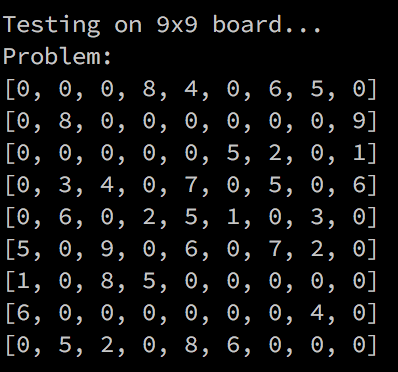
\includegraphics[width=70mm]{img/sudoku.png}
 \end{center}
 \caption{数独問題の例}
 \label{fig:one}
\end{minipage}
\begin{minipage}{0.5\hsize}
 \begin{center}
  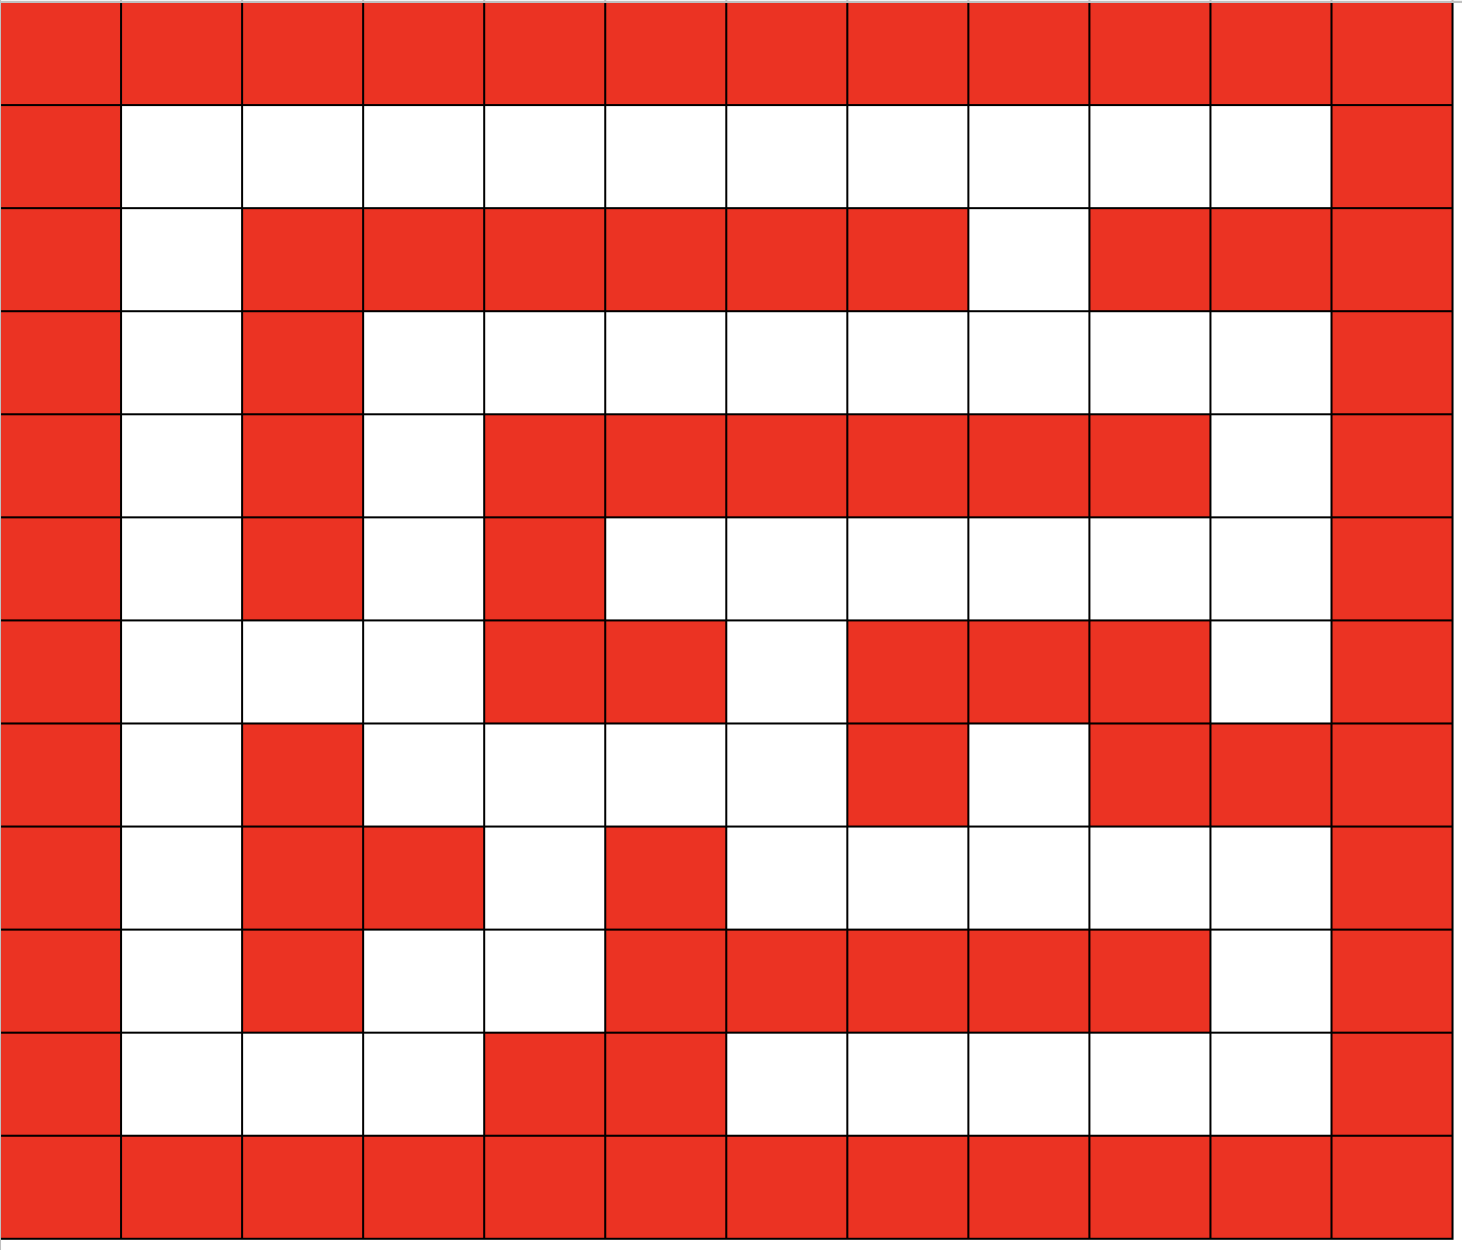
\includegraphics[width=70mm]{img/maze.png}
 \end{center}
 \caption{迷路問題の例}
 \label{fig:two}
\end{minipage}
\end{figure}


\subsection{数独の探索アルゴリズム}
数独の探索プログラムについてはsudokuディレクトリ以下にまとめて配置されており、
以下のコマンドをターミナルで実行することにより、幅優先探索、深さ優先探索
A*探索の実行及び結果の確認ができる。
\begin{lstlisting}[basicstyle=\ttfamily\footnotesize, frame=single]
  $ python3 sudoku.py
\end{lstlisting}

\subsubsection{幅優先探索アルゴリズムの実装について}
幅優先探索では解を求めるために木もしくはグラフの全てのノードを網羅的に探索、走査するするアルゴリズムであり、
以下の手順で探索を行う。
\begin{enumerate}
  \item 初めのノードを空のQueueに追加する。
  \item ノードをQueueの最初から取り出し、ノードが得たい結果であれば探索をやめて結果を返すが、
  そうでなければノードの全ての未探索の子をQueueに追加する。
  \item Queueが空になればグラフの全てのノードを探索したことを意味するため、探索をやめる。
\end{enumerate}

以下に数独問題における幅優先探索のプログラムを示す。node.expand(problem)により、
あるノードから数独問題の制約条件を満たし、実現可能なノードを得ることができ、
仮にこれらの子ノードの一つが目標状態を実現していれば、すなわち全てのマスが1から9までの数字で埋められて入れば
探索をやめ、そうでなければ全ての子ノードをQueueであるfrontierに追加してる。

\begin{lstlisting}[basicstyle=\ttfamily\footnotesize, frame=single]
  def BFS(problem):
      # Create initial node of problem tree holding original board
      node = Node(problem.initial)
      # Check if original board is correct and immediately return if valid
      if problem.goal_test(node.state):
          return node

      frontier = Queue()
      frontier.put(node)

      visited_node_num = 0
      while (frontier.qsize() != 0):
          node = frontier.get()
          for child in node.expand(problem):
              visited_node_num += 1
              if problem.goal_test(child.state):
                  print ("Found solution")
                  print("The number of visited nodes : " + str(visited_node_num))

                  return child
              frontier.put(child)
      return None
\end{lstlisting}

\subsubsection{深さ優先探索アルゴリズムの実装について}
深さ優先探索は木もしくはグラフのの最初のノードから、目的のノードが見つかるか、葉(子のないノード)に行く着くまで
深く探索をすすめ、その後はバックトラックし、最も近くの探索の終わっていないノードまで戻る。
ノードはStackに格納される。
\begin{enumerate}
  \item 初めのノードを空のStackに積む。
  \item ノードをStackの最初から取り出し(一番最近追加したノードが取り出される)、
  Nodeが得たい結果であれば探索をやめて結果を返すが、
  そうでなければノードに接続した子ノードをスタックに積み、これ以上子ノードを持たなくなるまで深く探索を進める。
  \item 子ノードを持たないノードに到達した際には、未訪問のノードまで戻る
  \item Stack空になればグラフの全てのノードを探索したことを意味するため、探索をやめる。
\end{enumerate}

以下に数独問題における深さ優先探索のプログラムを示す。最初のノードをスタックに追加し、
スタックの一番上のノードを取り出してそれが目標状態であれば探索をやめ、そうでなければ
そのノードから到達可能な小ノードをスタックについてし、目標状態に到達するもしくはスタックが空になるまで
探索を続ける。
\begin{lstlisting}[basicstyle=\ttfamily\footnotesize, frame=single]
  def DFS(problem):
  	initial_node = Node(problem.initial)
  	if problem.goal_test(initial_node.state):
  		return initial_node.state

  	stack = []
  	stack.append(initial_node)

  	visited_node_num = 0
  	while stack:
  		node = stack.pop()
  		visited_node_num+=1
  		if problem.goal_test(node.state):
  			print ("Found solution")
  			print("The number of visited nodes : " + str(visited_node_num))
  			return node.state
  		stack.extend(node.expand(problem))

  	return None
\end{lstlisting}

\subsubsection{A*探索アルゴリズムの実装について}
A*探索アルゴリズムとは、グラフ探索アルゴリズムの一つであり、グラフ上でスタートからゴールまでの道を見つけるというグラフ探索問題において、
ヒューリスティック関数を用いて探索を行うアルゴリズムである。ヒューリスティック関数をどう設定するかは問題によって異なる。
数独問題を解く上でヒューリスティックとなりうるとされるものにMinimum Remaining Values, Constraint Propagation
等があるが、今回はMinimum Remaining Valuesをヒュースティックと用いた。

Minimum Remaining Valuesとは、ある状態から次に埋めるべきマス目を選ぶ際、
ランダムもしくはインデックス順で行うのではなく、「制約上、選択可能な数字が最も小さいものから順に、すなわち制約の
厳しいものから順に選択する」というものである。
図3の例を用いてMinimum Remaining Valuesについて説明する。図において、
青いセルは行で見たときに既に1, 2が使用されており、またブロックで見たときに既に3が使用されており、
制約を満たす選択肢は4のみである。一方、赤色のセルは行、列、ブロックいずれで見ても他の数字がまだ使用されておらず、
1,2,3,4の全ての数字が利用可能であり、制約を満たす選択肢は4つ存在する。よって青のセルの方がremaining values
が小さくなるために、次に選択されるのは青のセルとなる。

\begin{figure}
  \begin{center}
    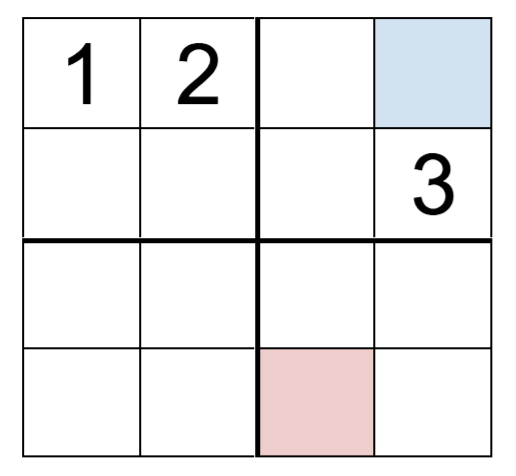
\includegraphics[width=6cm]{img/sudok_minimu.png}
    \caption{Minimum Remaining Valuesの例}
  \end{center}
\end{figure}

A*探索法については、Minimum remaining valuesをヒューリスティックとし、次に埋めるセルを選択する際、
これが最小となるものを次のセルとして選択、有効な数字のうち最小のものでそのセルを埋めるという方式をとった。

\begin{lstlisting}[basicstyle=\ttfamily\footnotesize, frame=single]
# Calcumate minimum remaining values for each cell.
def heuristic(self, board, state):
    min_remainings = [
        [self.type + 1 for i in range(1, self.type + 1)] for i in range(1, self.type + 1)]
    for row in range(board):
        for column in range(board):
            if state[row][column] == 0:
                valid_nums = self.filter_quad(self.filter_column(
                    self.filter_row(state, row), state, column), state, row, column)
                min_remainings[row][column] = len(valid_nums)
    return min_remainings

# Get an empty spot with a heuristic.
def get_spot(self, board, state):
    min_remainings = self.heuristic(board, state)

    minimum = np.array(min_remainings).min()
    for row in range(board):
        for column in range(board):
            if min_remainings[row][column] == minimum and state[row][column] == 0:
                return row, column

def AStar(problem):
    initial_node = Node(problem.initial)
    if problem.goal_test(initial_node.state):
        return initial_node.state

    stack = []
    stack.append(initial_node)

    visited_node_num = 0
    while stack:
        node = stack.pop()
        visited_node_num += 1
        if problem.goal_test(node.state):
            return node.state
        stack.extend(node.expand(problem))

    return None

\end{lstlisting}


\subsection{迷路の探索アルゴリズム}
迷路の探索プログラムについては、mazeディレクトリ以下、主に$\rm{maze\_solver.py}$というファイルに
幅優先探索、深さ優先探索、A*探索のプログラムが記述されており、以下のコマンドで実行及び結果の確認ができる。

\begin{lstlisting}[basicstyle=\ttfamily\footnotesize, frame=single]
  $ python3 maze.py
\end{lstlisting}

この迷路においてグラフは辞書型で表されており、i行j列のセルに隣接するセルの情報がこのグラフ辞書の(i, j)
というキーに対応した値となる。またこの値は隣接するセルのインデックスと接続している邦楽のタプルで与えられる。
例えば図4のような迷路をグラフに落とし込むとする。
\begin{figure}
  \begin{center}
    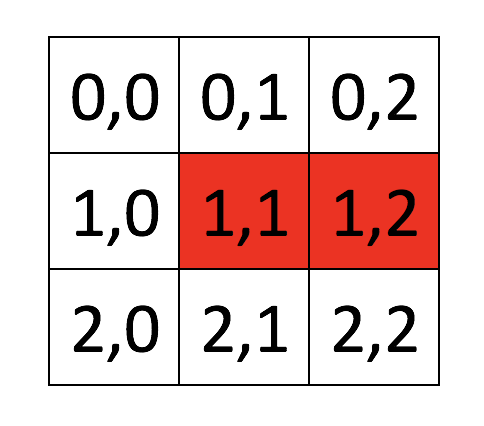
\includegraphics[width=6cm]{img/maze_graph.png}
    \caption{迷路のグラフ表現の例}
  \end{center}
\end{figure}
1行0列のマスは南北のセルからは行き来が可能だが、東西側は両方とも行き止まりないしは壁になるため、隣接しているとは
言えない。よってこのセルのグラフ辞書での値は以下の通りになる。
\begin{lstlisting}[basicstyle=\ttfamily\footnotesize, frame=single]
  graph[1][0] = [("S", (2, 0)), ("N", (0, 0))]
\end{lstlisting}
このように構成されたグラフ辞書に基づいて、探索を行う。

\subsubsection{幅優先探索アルゴリズムの実装について}
幅優先探索については、sudokuの場合と同様、Queueを使用し、あらかじめ設定されたgoal地点に到達すれば終了、
そうでなければQueueから新たに取り出し、取り出されたノードから移動可能な全てのノードを新たにQueueに追加し
これをQueueが空になるまで続ける。

\begin{lstlisting}[basicstyle=\ttfamily\footnotesize, frame=single]
def solve_bfs(maze, graph):
    start, goal = (1, 1), (len(maze) - 2, len(maze[0]) - 2)
    queue = deque([("", start)])
    visited = set()
    while queue:
        path, current = queue.popleft()
        if current == goal:
            return path
        if current in visited:
            continue
        visited.add(current)
        for direction, neighbour in graph[current]:
            queue.append((path + direction, neighbour))
    return "Cannot find any way."

\end{lstlisting}

\subsubsection{深さ優先探索アルゴリズムの実装について}
深さ優先探索プログラムも数独問題と同様、Stackを利用し、Stackが空になるもしくは
ゴールに到達するまで探索を続ける。

\begin{lstlisting}[basicstyle=\ttfamily\footnotesize, frame=single]
def solve_dfs(maze, graph):
    start, goal = (1, 1), (len(maze) - 2, len(maze[0]) - 2)
    stack = deque([("", start)])
    visited = set()
    while stack:
        path, current = stack.pop()
        if current == goal:
            return path
        if current in visited:
            continue
        visited.add(current)
        for direction, neighbour in graph[current]:
            stack.append((path + direction, neighbour))
    return "Cannot find any way."
\end{lstlisting}

\subsubsection{A*探索アルゴリズムの実装について}
迷路問題におけるA*探索アルゴリズムは、ダイクストラ法を用いてスタート地点からゴール地点へ
最も少ないコストで到達可能な経路を見つける音を目指す。実相においてはあるセルから
ゴール地点までの距離をヒューリスティックとして用い、Priority Queueに可能な経路の
情報を追加、削除していく。

\begin{lstlisting}[basicstyle=\ttfamily\footnotesize, frame=single]
def heuristic(cell, goal):
    return abs(cell[0] - goal[0]) + abs(cell[1] - goal[1])

def solve_astar(maze, graph):
    start, goal = (1, 1), (len(maze) - 2, len(maze[0]) - 2)
    pr_queue = []
    heappush(pr_queue, (0 + heuristic(start, goal), 0, "", start))
    visited = set()
    while pr_queue:
        _, cost, path, current = heappop(pr_queue)
        if current == goal:
            return path
        if current in visited:
            continue
        visited.add(current)
        for direction, neighbour in graph[current]:
            heappush(pr_queue, (cost + heuristic(neighbour, goal), cost + 1,
                                path + direction, neighbour))
    return "Cannot find any way."

\end{lstlisting}

\section{探索の効率性に関する結果と考察}
\subsection{数独問題についての結果の考察}
4つの数独問題について、探索法ごとに正解に到達するまでに探索したノードの数を比較したものが
次の表1である。
\begin{figure}[htbp]
 \begin{minipage}{0.5\hsize}
  \begin{center}
   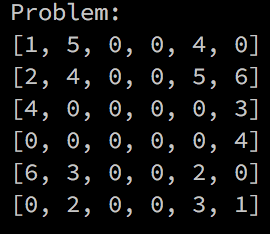
\includegraphics[width=70mm]{img/sudoku_1.png}
  \end{center}
  \caption{数独 問題1}
  \label{fig:one}
 \end{minipage}
 \begin{minipage}{0.5\hsize}
  \begin{center}
   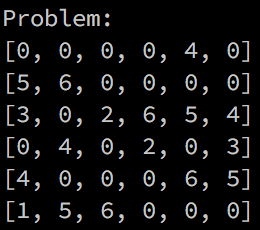
\includegraphics[width=70mm]{img/sudoku_2.png}
  \end{center}
  \caption{数独 問題2}
  \label{fig:two}
 \end{minipage}
\end{figure}
\begin{figure}[htbp]
 \begin{minipage}{0.5\hsize}
  \begin{center}
   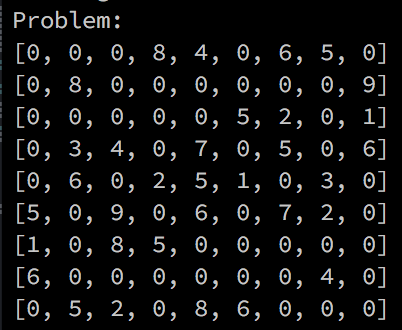
\includegraphics[width=70mm]{img/sudoku_3.png}
  \end{center}
  \caption{数独 問題3}
  \label{fig:one}
 \end{minipage}
 \begin{minipage}{0.5\hsize}
  \begin{center}
   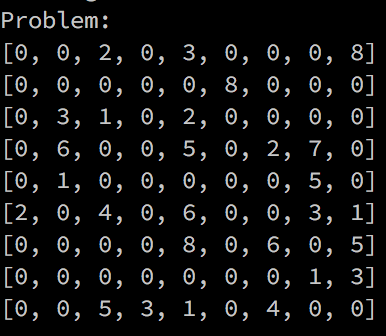
\includegraphics[width=70mm]{img/sudoku_4.png}
  \end{center}
  \caption{数独 問題4}
  \label{fig:two}
 \end{minipage}
\end{figure}
表から数独問題のサイズが大きくなるほど、より多くの手が想定できるために、幅優先探索、
深さ優先探索では指数的に探索するノードの数が増加していることがわかり、特に幅優先探索については
この傾向が顕著であることがわかる。一方A*探索は問題のサイズが大きくなったとしても
探索するノードの数は他の二つと比較してそこまで増加はしておらず、ヒューリスティックを用いいることにより、
より効率的な探索・走査ができていることがわかる。

\begin{table}[htb]
  \begin{center}
      \caption{DFS, BFS, A*により探索したノード数比較}
  \begin{tabular}{|c|c|c|c|} \hline
    問題番号 & 幅優先探索 & 深さ優先探索 & A*探索\\  \hline \hline
    1 & 78 & 23 & 21 \\
    2 & 48 & 20 & 20 \\
    3 & 1932 & 939 & 49 \\
    4 & 285352 & 16427 & 410 \\
    \hline
  \end{tabular}
  \end{center}
\end{table}

\subsection{迷路問題についての結果の考察}
迷路問題については、次の二つの問題について幅優先探索、深さ優先探索、A*探索により解法を求めた。
\begin{figure}[htbp]
 \begin{minipage}{0.5\hsize}
  \begin{center}
   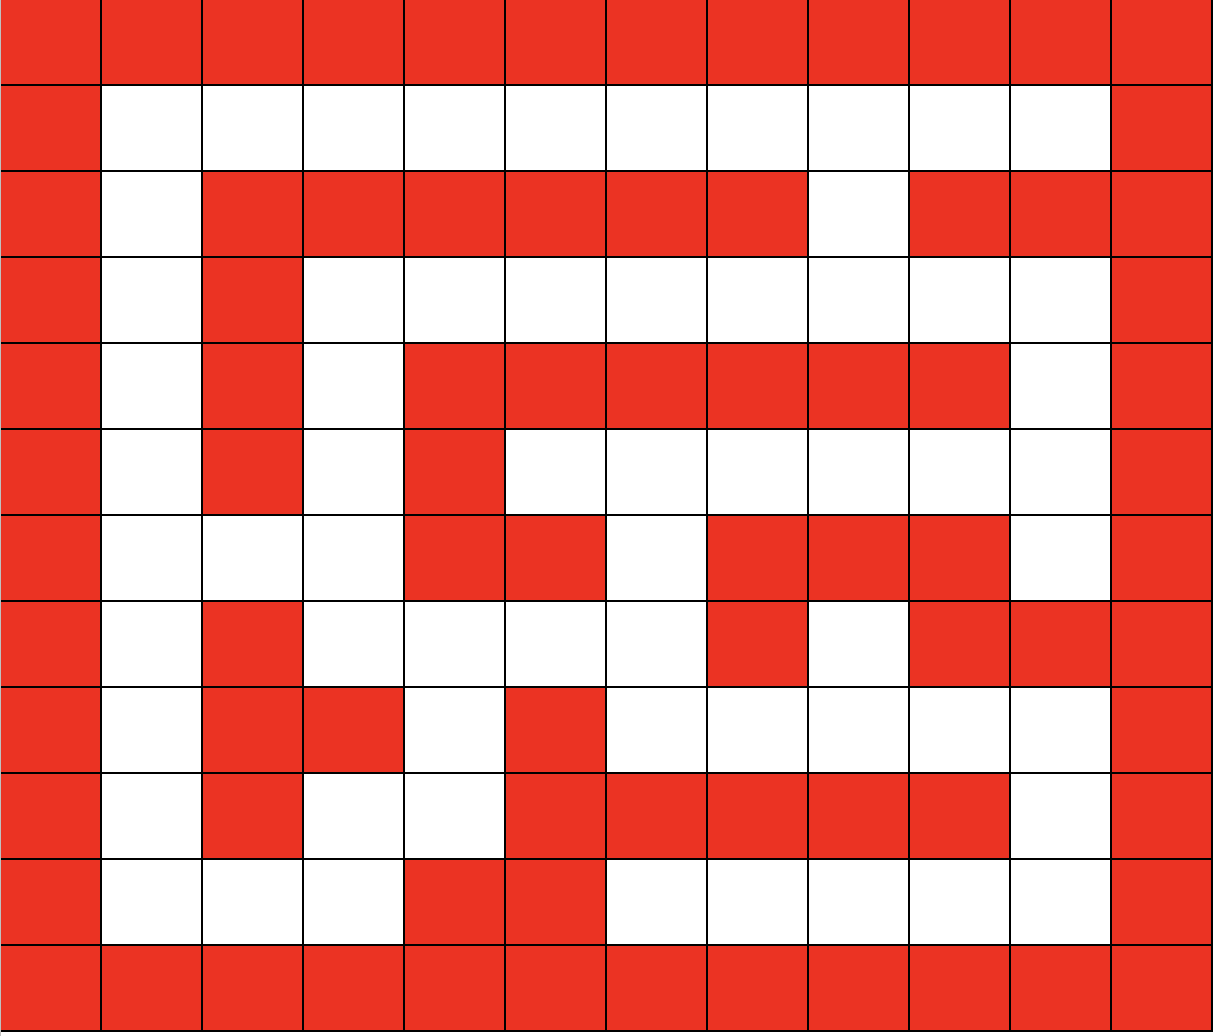
\includegraphics[width=70mm]{img/maze_1.png}
  \end{center}
  \caption{迷路問題1}
  \label{fig:one}
 \end{minipage}
 \begin{minipage}{0.5\hsize}
  \begin{center}
   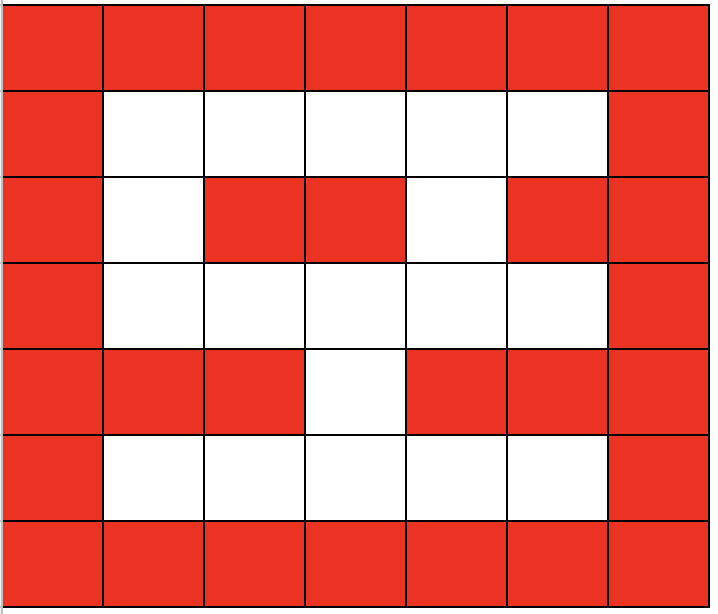
\includegraphics[width=70mm]{img/maze_2.png}
  \end{center}
  \caption{迷路問題2}
  \label{fig:two}
 \end{minipage}
\end{figure}
どちらの問題についても、深さ優先探索とA*探索問題で得られた経路は一致し、また幅優先探索の導いた経路と比較し、
問題1は距離が7、問題2は距離が2、幅優先探索の結果得られた経路より短くなった。
問題1の解法は図11及び図12、問題2の解放は図13及び14で確認できる。

\begin{figure}[htbp]
 \begin{minipage}{0.5\hsize}
  \begin{center}
   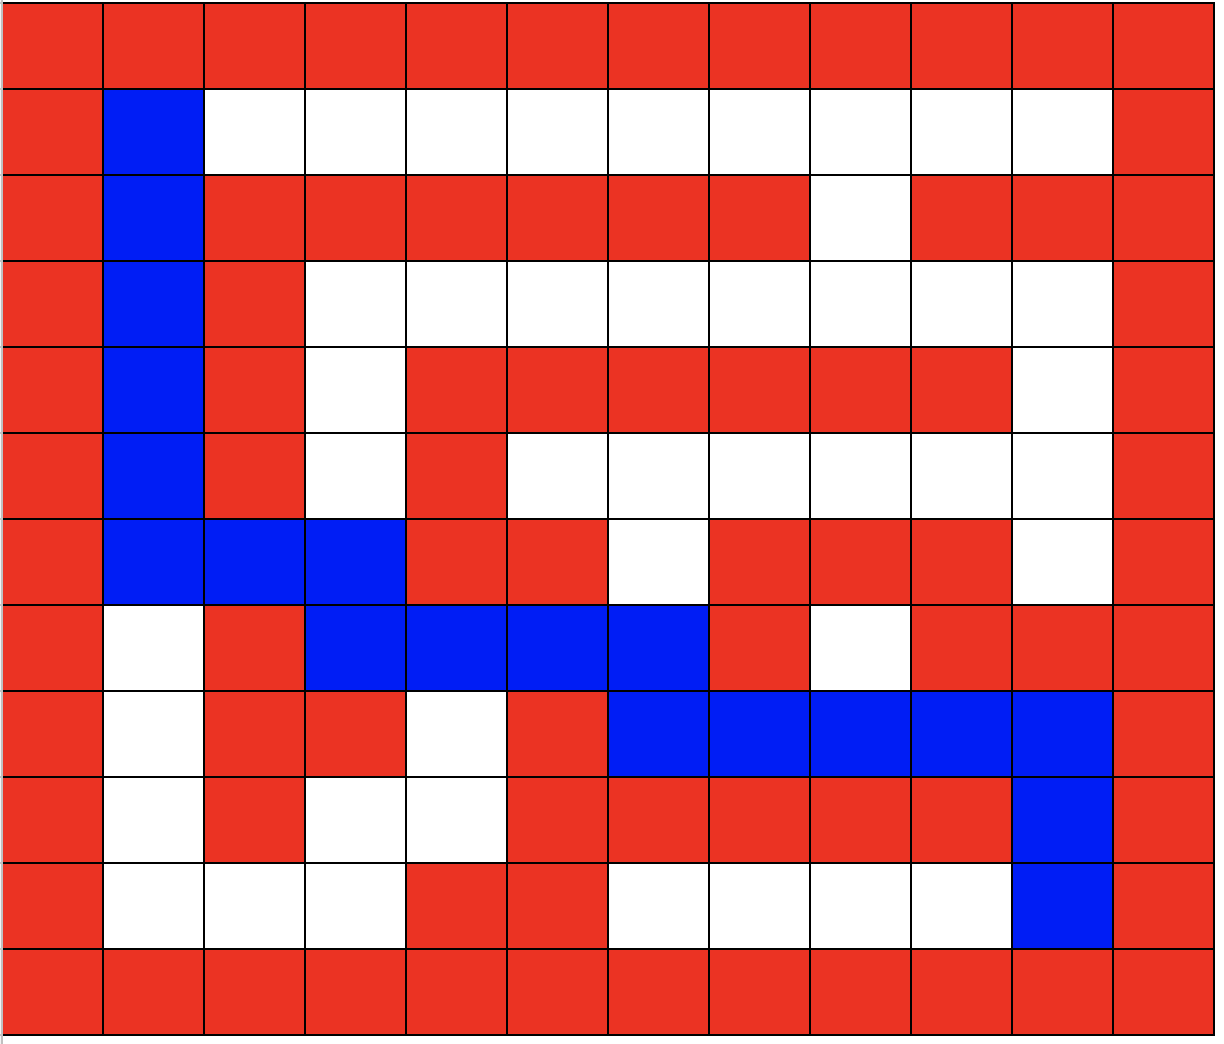
\includegraphics[width=70mm]{img/maze_1_dfs_astar.png}
  \end{center}
  \caption{迷路問題1 深さ優先探索、A*探索の結果得られた経路}
  \label{fig:one}
 \end{minipage}
 \begin{minipage}{0.5\hsize}
  \begin{center}
   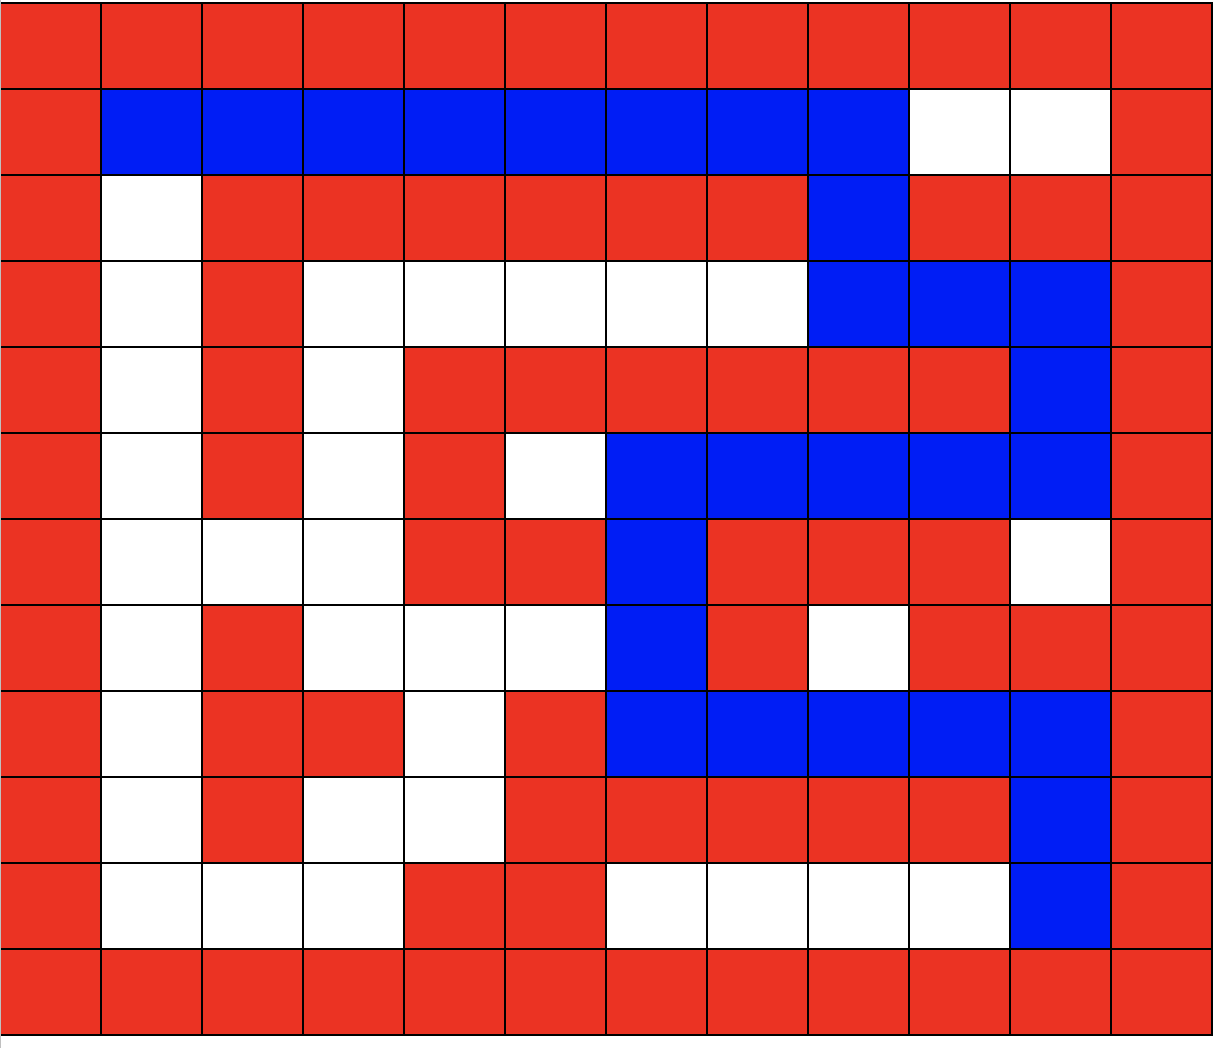
\includegraphics[width=70mm]{img/maze_1_bfs.png}
  \end{center}
  \caption{迷路問題1 幅優先探索の結果得られた経路}
  \label{fig:two}
 \end{minipage}
\end{figure}

\begin{figure}[htbp]
 \begin{minipage}{0.5\hsize}
  \begin{center}
   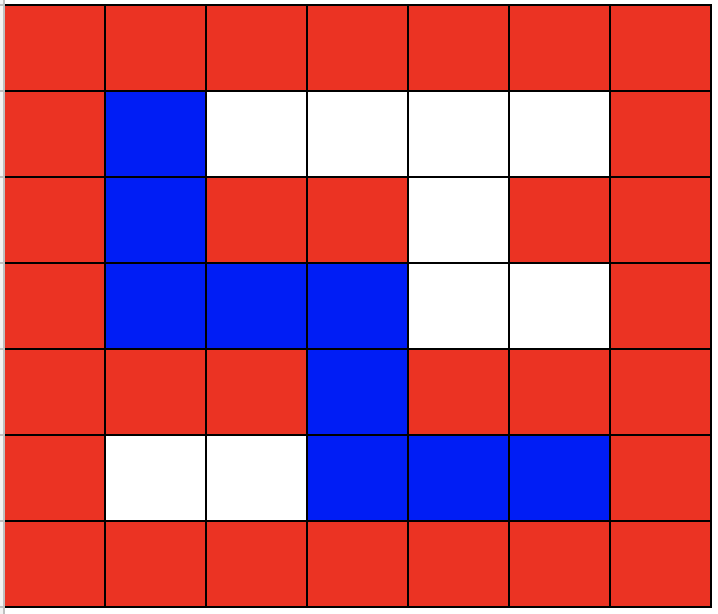
\includegraphics[width=70mm]{img/maze_2_dfs.png}
  \end{center}
  \caption{迷路問題2 深さ優先探索、A*探索の結果得られた経路}
  \label{fig:one}
 \end{minipage}
 \begin{minipage}{0.5\hsize}
  \begin{center}
   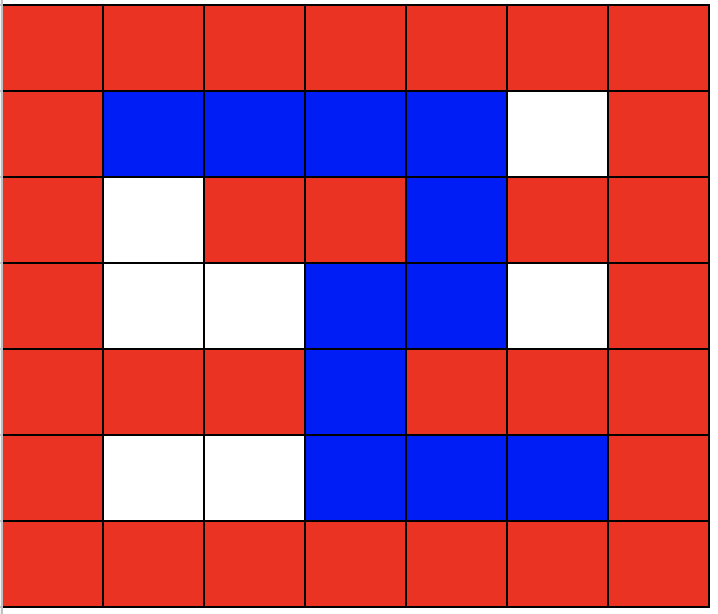
\includegraphics[width=70mm]{img/maze_2_bfs.png}
  \end{center}
  \caption{迷路問題2 幅優先探索の結果得られた経路}
  \label{fig:two}
 \end{minipage}
\end{figure}

この経路を得るために探索したノードの数は以下の通りである。表2より結果として深さ優先探索は最短経路を求められてはいる一方で、
探索するノードの数が迷路のサイズの上昇とともに他の二つの探索法を比較して、大きく増加していることがわかる。一方A*探索は
深さ優先探索と同様の解を導きつつも、迷路のサイズが増加しても探索数はさほど増加せず、大きく、かつある程度分岐可能性の存在する
迷路においては、ヒューリスティックを活用したA*探索法がより効率的により短い経路を探索するのに有効であることがわかる。

\begin{table}[htb]
  \begin{center}
    \caption{迷路問題においてDFS, BFS, A*により探索したノード数比較}
  \begin{tabular}{|c|c|c|c|} \hline
    問題番号 & 幅優先探索 & 深さ優先探索 & A*探索\\  \hline \hline
    1 & 38 & 120 & 43 \\
    2 & 17 & 35 & 17 \\
    \hline
  \end{tabular}
  \end{center}
\end{table}

\begin{thebibliography}{9}
  \bibitem{evans} Thomas H. Cormen, Charles E. Leiserson, Ronald L. Rivest, Clifford Stein.
    "Introduction to Algorithms", MIT Press, 2009.
  \bibitem{iba} 伊庭斉志,
    『人工知能と人工生命の基礎』, オーム社 , 2013.
\end{thebibliography}


\end{document}
